\documentclass[11pt,a4paper]{article}

\usepackage[utf8]{inputenc}
\usepackage[T1]{fontenc}
\usepackage[spanish,es-nodecimaldot]{babel}
\usepackage{amsmath}
\usepackage{booktabs}
\usepackage{tabularx}
\usepackage{graphicx}
\usepackage{geometry}
\usepackage{xcolor}
\usepackage{hyperref}
\geometry{margin=2.2cm}

\hypersetup{
    colorlinks=true,
    linkcolor=blue!50!black,
    citecolor=blue!50!black,
    urlcolor=blue!50!black,
    pdftitle={Reporte de reproducibilidad residual multi-seed},
    pdfauthor={Cesar Zapata}
}

\newcolumntype{Y}{>{\raggedright\arraybackslash}X}

\title{Reporte de reproducibilidad residual multi-seed\\\large Proyecto TD3 para pr\'otesis mioel\'ectrica}
\author{C\'esar Zapata\\Research Laboratory in Artificial Intelligence and Computer Vision ``Alan Turing''}
\date{30 de marzo de 2026}

\begin{document}
\maketitle

\section*{Prop\'osito}
Este reporte documenta la nueva fase de reproducibilidad a\~nadida despu\'es del resultado residual de una sola corrida. El objetivo inmediato fue responder una pregunta natural de revisi\'on: si la mejora residual observada en el mejor checkpoint individual, \texttt{Agent1850}, se mantiene cuando la misma receta residual se entrena con m\'ultiples semillas aleatorias.

\section*{Por qu\'e se a\~nadi\'o esta fase}
La versi\'on anterior del paper era fuerte como reporte de proyecto, pero segu\'ia siendo vulnerable a una cr\'itica estad\'istica est\'andar: la afirmaci\'on final del residual depend\'ia de una sola corrida exitosa. Para reducir esa debilidad, el repositorio se extendi\'o con:
\begin{itemize}
    \item control expl\'icito de la semilla aleatoria durante el entrenamiento;
    \item un launcher multi-seed para el m\'etodo residual;
    \item agregaci\'on autom\'atica de las m\'etricas finales entre seeds;
    \item una figura de estilo acad\'emico que resume el resultado multi-seed.
\end{itemize}

\section*{Protocolo experimental}
La campa\~na multi-seed us\'o el mismo benchmark validado y la misma receta residual que antes produjo el mejor resultado individual.

\begin{table}[h!]
\centering
\caption{Configuraci\'on fija de la campa\~na residual multi-seed}
\begin{tabularx}{\linewidth}{lY}
\toprule
Elemento & Valor \\
\midrule
Checkpoint base congelado & \texttt{Agent7250\_valid\_baseline.mat} \\
M\'etodo residual & Residual Lift \\
Escala residual & $\alpha_{\mathrm{res}} = 0.20$ \\
Ancho oculto residual & 32 \\
Exploraci\'on std/min/decay & $0.02 / 0.002 / 10^{-4}$ \\
Episodios de entrenamiento por seed & 2000 \\
Guardado de checkpoints & cada 50 episodios \\
Pol\'itica de auditor\'ia & cola cada 50 en los \'ultimos 12 checkpoints \\
Auditor\'ia r\'apida / completa & 20 / 50 simulaciones \\
Seeds & $\{11, 22, 33, 44, 55\}$ \\
Benchmark de referencia & \texttt{Agent7250} \\
\bottomrule
\end{tabularx}
\end{table}

Para cada seed, el flujo fue:
\begin{enumerate}
    \item entrenar una corrida residual independiente;
    \item auditar los checkpoints guardados;
    \item escoger el mejor checkpoint con la misma regla de ranking usada en fases anteriores;
    \item ejecutar la evaluaci\'on final de 50 simulaciones sobre ese checkpoint seleccionado.
\end{enumerate}

\section*{Resultados principales}
El resumen agregado final de la campa\~na multi-seed se muestra en la Tabla~\ref{tab:aggregate}. Los valores benchmark corresponden al checkpoint can\'onico \texttt{Agent7250}.

\begin{table}[h!]
\centering
\caption{Resultado agregado de la campa\~na residual de cinco seeds}
\label{tab:aggregate}
\begin{tabularx}{\linewidth}{lYY}
\toprule
M\'etrica & Benchmark (\texttt{Agent7250}) & Residual multi-seed media $\pm$ desviaci\'on \\
\midrule
trackingMSE & 0.043045 & 0.043785 $\pm$ 0.001517 \\
trackingMAE & 0.160336 & 0.161675 $\pm$ 0.002406 \\
actionL2 & 0.596444 & 0.581119 $\pm$ 0.069363 \\
saturationFraction & 0.392086 & 0.336202 $\pm$ 0.147114 \\
deltaActionL2 & 0.321385 & 0.344544 $\pm$ 0.036101 \\
\bottomrule
\end{tabularx}
\end{table}

\begin{table}[h!]
\centering
\caption{Resultado final por seed}
\begin{tabularx}{\linewidth}{c c c c c c}
\toprule
Seed & Estado & Mejor episodio & trackingMSE & actionL2 & saturationFraction \\
\midrule
11 & Rejected & 1850 & 0.046020 & 0.461390 & 0.084744 \\
22 & ConditionA & 1850 & 0.043045 & 0.582150 & 0.337480 \\
33 & Rejected & 1600 & 0.044557 & 0.609480 & 0.380300 \\
44 & Rejected & 1850 & 0.043157 & 0.622773 & 0.430408 \\
55 & Rejected & 1850 & 0.042149 & 0.629797 & 0.448081 \\
\bottomrule
\end{tabularx}
\end{table}

La figura resumen generada para esta fase se muestra en la Fig.~\ref{fig:multiseed}.

\begin{figure}[h!]
\centering
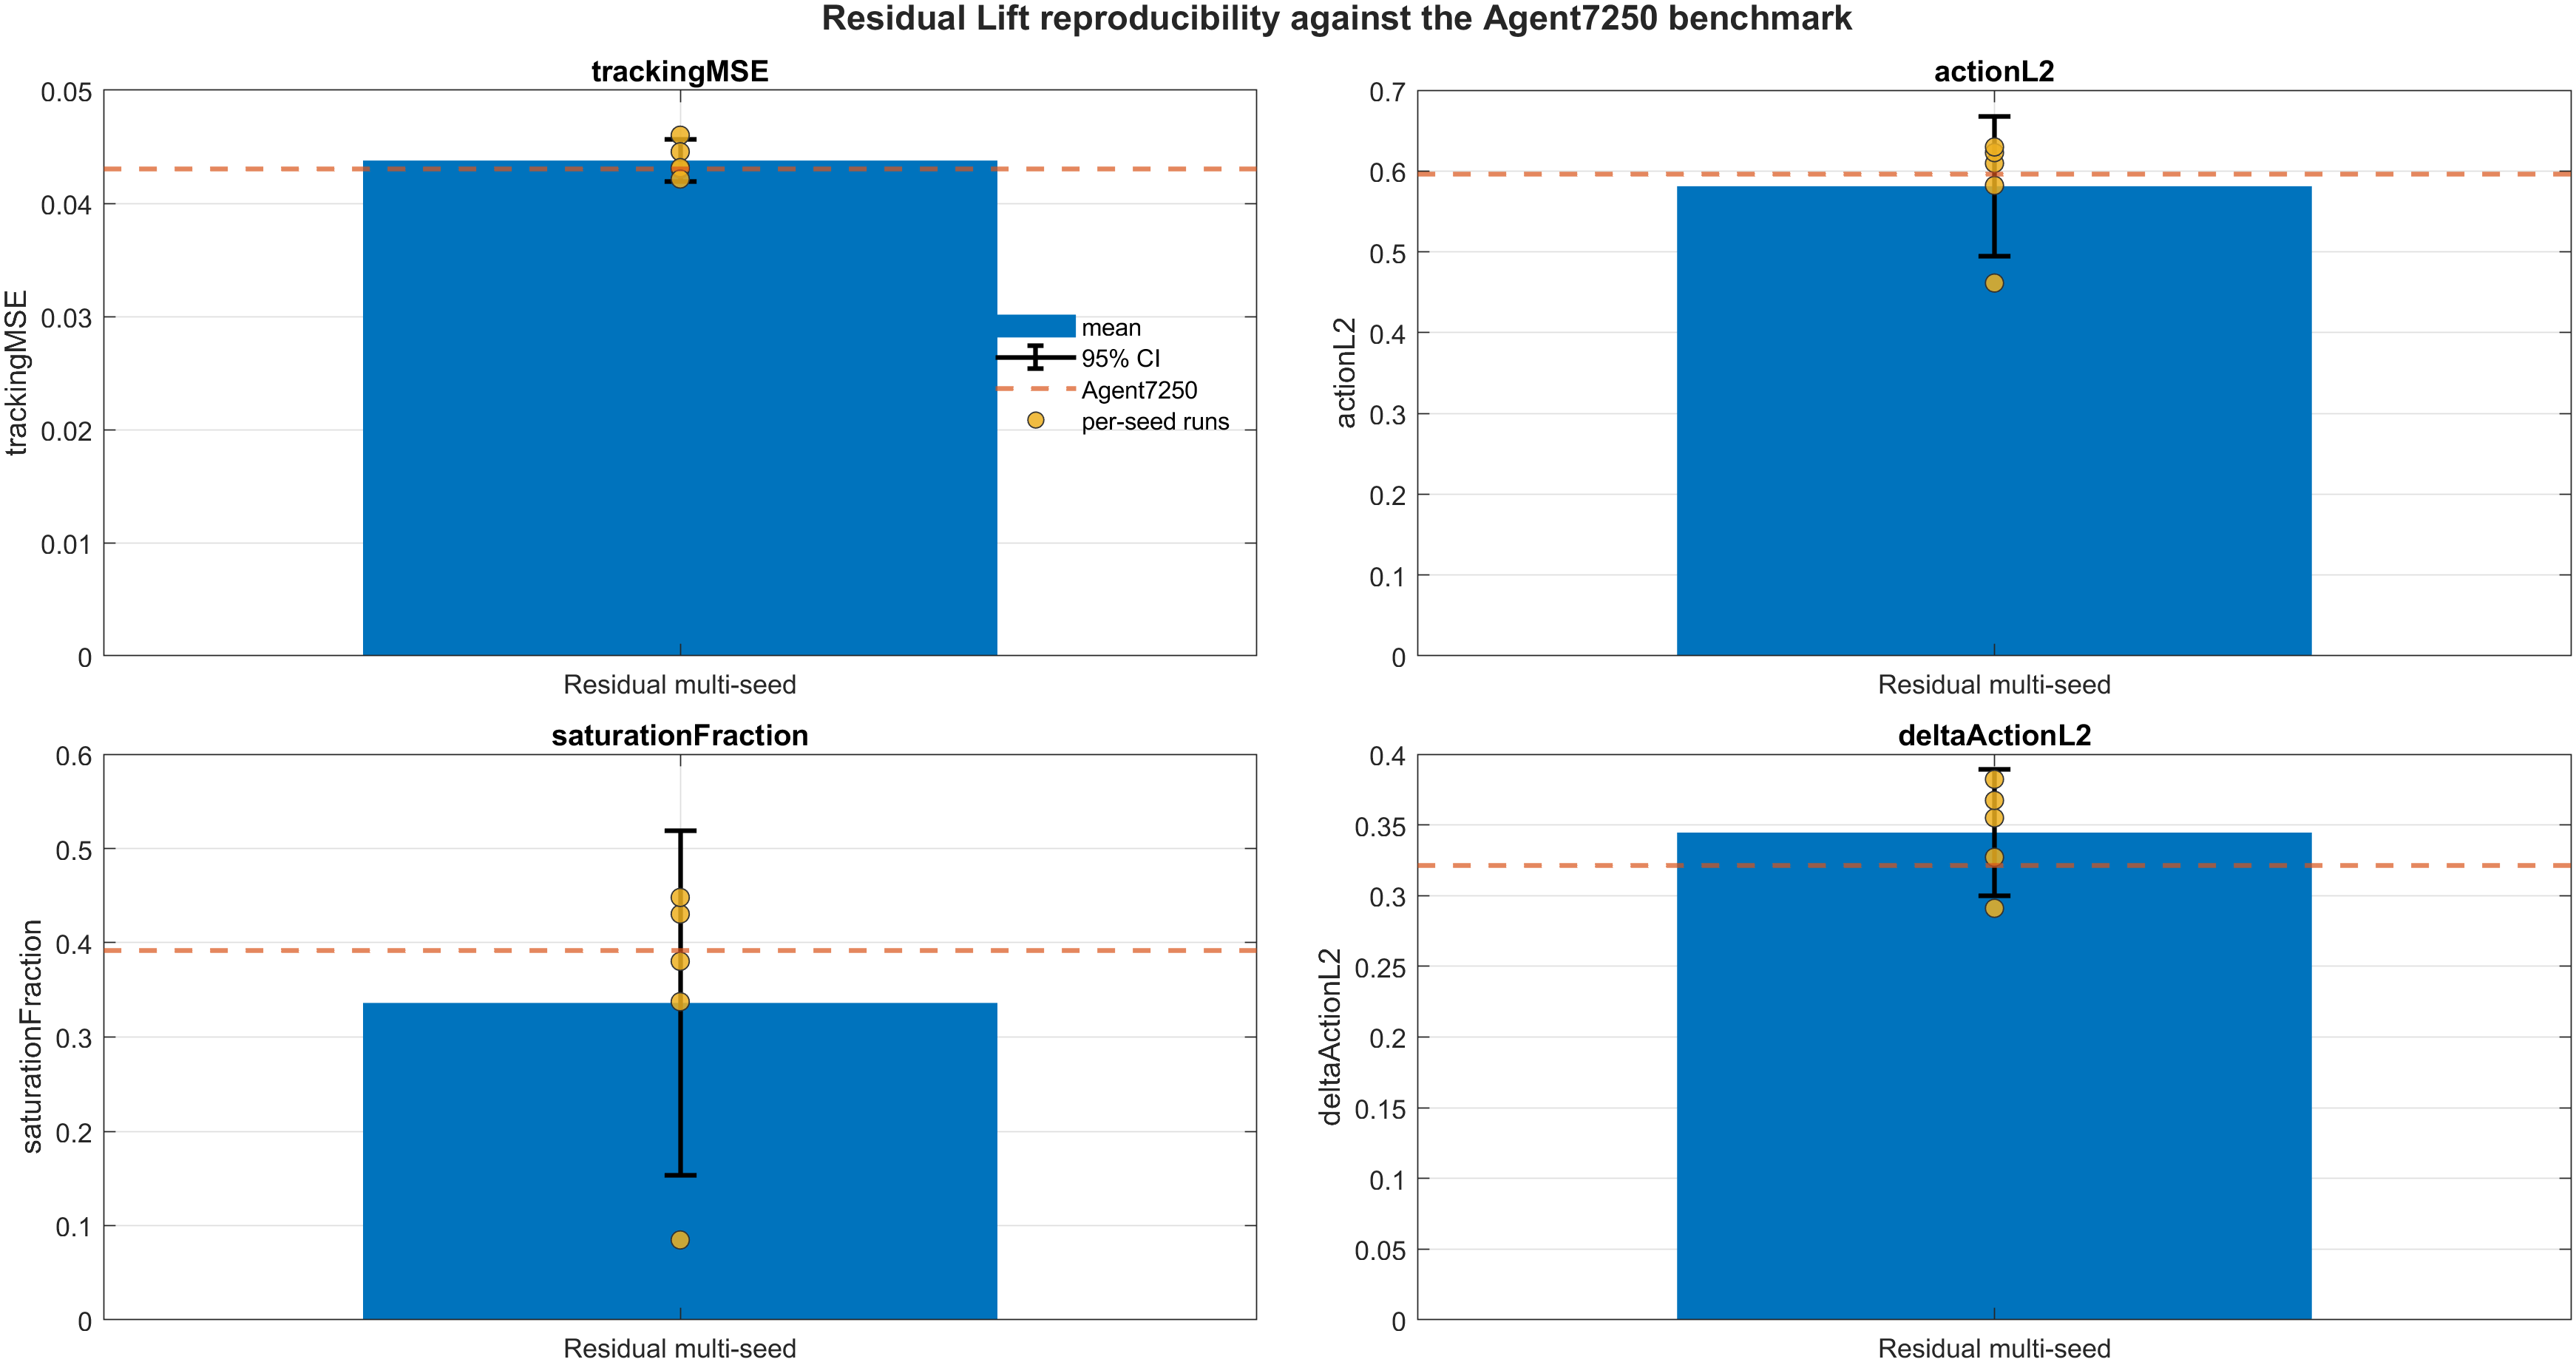
\includegraphics[width=\linewidth]{figures/residual_multiseed_summary_20260330.png}
\caption{Resumen visual de la reproducibilidad residual. La l\'inea punteada representa el benchmark, la barra muestra la media de las cinco seeds, el whisker negro muestra el intervalo de confianza del 95\% y los puntos corresponden a las seeds individuales.}
\label{fig:multiseed}
\end{figure}

\section*{Interpretaci\'on}
Esta fase cambi\'o de manera importante la fuerza del claim del proyecto.

\subsection*{Lo que s\'i mejor\'o}
\begin{itemize}
    \item El repositorio ahora puede producir evidencia de corridas repetidas y no solo un checkpoint exitoso aislado.
    \item La campa\~na multi-seed confirma que la familia residual sigue siendo la \'unica l\'inea post-benchmark que ha producido una corrida repetida aceptada contra el benchmark.
    \item La seed 22 reprodujo el mejor comportamiento aceptado y cumpli\'o \texttt{ConditionA}.
\end{itemize}

\subsection*{Lo que no mejor\'o}
\begin{itemize}
    \item El beneficio residual todav\'ia no es estad\'isticamente estable entre seeds.
    \item Solo 1 de las 5 seeds cumpli\'o la regla de aceptaci\'on contra el benchmark.
    \item La media agregada ya no sostiene la narrativa fuerte de una mejora robusta, porque el \texttt{trackingMSE} empeora ligeramente y \texttt{deltaActionL2} tambi\'en empeora en promedio.
    \item La dispersi\'on de \texttt{saturationFraction} sigue siendo amplia, lo que muestra sensibilidad fuerte de la l\'inea residual al reentrenamiento.
\end{itemize}

\subsection*{Qu\'e significa esto para el paper}
La l\'inea residual sigue siendo la m\'as prometedora y la m\'as interesante cient\'ificamente dentro del repositorio. Sin embargo, despu\'es de la campa\~na multi-seed, la afirmaci\'on m\'as defendible ya no es ``el m\'etodo residual mejora robustamente el benchmark''. La afirmaci\'on m\'as honesta y fuerte ahora es:
\begin{quote}
el m\'etodo residual produjo la mejor pol\'itica individual del proyecto, y una de las cinco corridas repetidas reprodujo un controlador aceptado contra el benchmark, pero la evidencia entre corridas todav\'ia muestra variabilidad importante.
\end{quote}

\section*{Entregables generados en esta fase}
Esta fase produjo:
\begin{itemize}
    \item un nuevo launcher multi-seed en el c\'odigo MATLAB;
    \item archivos de resumen por seed y agregados en la carpeta de resultados experimentales;
    \item una figura de estilo publicaci\'on para el paper;
    \item una versi\'on revisada del paper IEEE con detalles de dataset, limitaciones y lenguaje de reproducibilidad.
\end{itemize}

\section*{Conclusi\'on}
La nueva fase multi-seed fue exitosa como mejora metodol\'ogica, aunque debilit\'o el claim fuerte del residual como sustituto robusto del benchmark. Esto fortalece el proyecto porque reemplaza un resultado final anecd\'otico por una evaluaci\'on repetida y m\'as defendible. El resultado pr\'actico es doble: el mejor checkpoint residual individual sigue siendo importante como mejor \emph{single-run}, pero ahora el proyecto tambi\'en tiene una visi\'on m\'as realista de cu\'an sensible es esa mejora al reentrenamiento.

\end{document}
